\section*{Problema 01}

\textbf{Calcule y clasifique los puntos críticos de la siguiente función}

\begin{equation*}
    f(x_1,x_2) = (x_1^2+x_2^2-1)^2+(x_2^2-1)^2
\end{equation*}

\textbf{Muestra la función usando python}


Se tiene que el gradiente de la función $f(x_1,x_2)$ es:

\begin{equation*}
    \nabla f(x_1x_2) = \begin{bmatrix}
        4x_1 (x_1^2+x_2^2-1) \\
        4x_2 (x_1^2+2x_2-2)
    \end{bmatrix}
\end{equation*}

y su hessiano es el siguiente:

\begin{equation*}
    \nabla^2 f(x_1,x_2) = \begin{bmatrix}
        12x_1+4x_2 -4 & 8x_1x_2      \\
        8x_1x_2       & 4x_1+24x_2-8
    \end{bmatrix}
\end{equation*}

Con el gradiente de $f(x_1,x_2)$ se pueden encontrar los valores críticos, los cuales son:

\begin{equation*}
    x_1 = 0 \qquad x_1^2+x_2^2=1 \qquad \rightarrow\qquad x_2 = -1,1
\end{equation*}

\begin{equation*}
    x_2 = 0 \qquad x_1^2+2x_2^2=2 \qquad \rightarrow \qquad x_1 = -1,1
\end{equation*}

por ende, los puntos críticos son $x=\{(0,0),(0,1),(0,-1),(1,0),(-1,0)\}$

Evualuando el hessiano con los puntos críticos se obtiene la siguiente tabla:

\begin{table}[H]
    \centering
    \begin{tabular}{cccccc} \hline
        \textbf{Punto crítico} & $(0,1)$                      & $(0,-1)$                     & $(1,0)$                      & $(-1,0)$                     & $(0,0)$                      \\  [0.125cm] \hline
        $\nabla^2 f(x)$        & $\begin{bmatrix} 0 & 0 \\  0 & 16\end{bmatrix} $ & $\begin{bmatrix} 0 & 0 \\  0 & 16\end{bmatrix} $ & $\begin{bmatrix} 8 & 0 \\  0 & -4\end{bmatrix} $ & $\begin{bmatrix} 8 & 0 \\  0 & -4\end{bmatrix} $ & $\begin{bmatrix} -4 & 0 \\  0 & -8\end{bmatrix}$ \\ \hline
    \end{tabular}
    \caption{Hessianos de cada punto crítico encontrado}
\end{table}

Con estos resultados se pueden obtener que los puntos $(0,1)$ y $(0,-1)$ son mínimos. Por el hecho que la función esta acotada para número mayores e iguales a cero y la función evaluada en estos puntos  es cero ($f(0,1)=f(0,-1)=0$) se afirma que estos dos puntos representan mínimos globales.

Por otro lado los puntos $(1,0)$ y $(-1,0)$ representan puntos silla debido a que su hessiano no es positivo definido.

Por ultimo el punto $(0,0)$ representa un máximo de la función y como la misma no tiene una cota superior, entonces este representa un máximo local.

En la figura \ref{fig} se ve representada la función con los puntos crítcos marcados con estrellas

\begin{figure}[H]
    \centering
    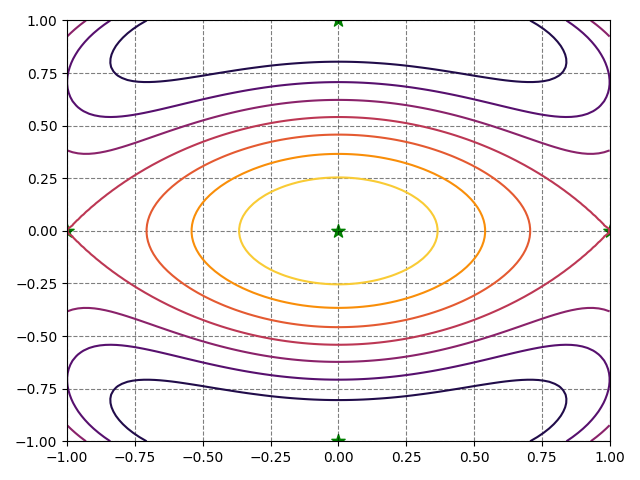
\includegraphics[width=16cm]{Graphics/Problema_01.png}
    \caption{}
    \label{fig}
\end{figure}